\chapter{Architektur}
%\chapter{\colorbox{yellow}{Architektur}}

\section{Konzept}
%\section{\colorbox{green}{Konzept}}

%\begin{wrapfigure}{l}{0.4\textwidth}
%\begin{center}
%\vspace{-40pt}%
% 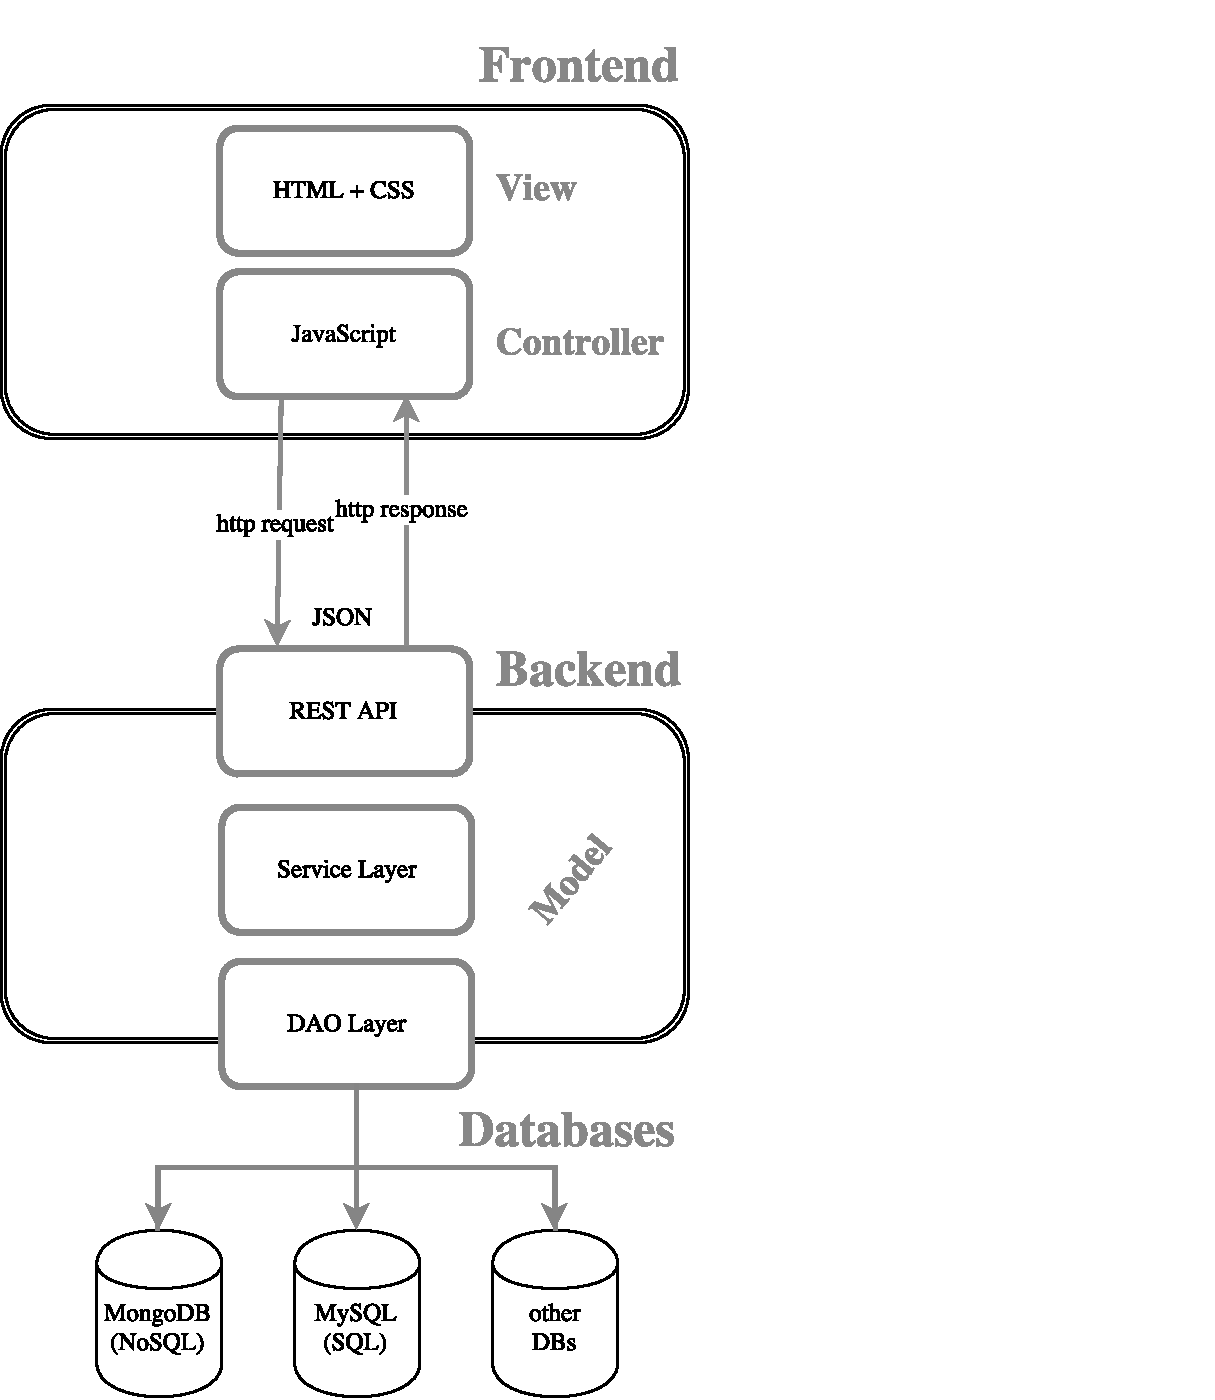
\includegraphics[trim = 0mm 0mm 0mm 0mm, clip, width=0.4\textwidth]{resources/architectureMyAppWithoutFrameworks}	
% \caption[Architektur-Prototyp]{Architektur-Prototyp}
% \label{img:architectureMyApp}
% \vspace{-70pt}%
% \end{center}
% \end{wrapfigure}

\begin{figure}[H]
\vspace{-30pt}%
\centering
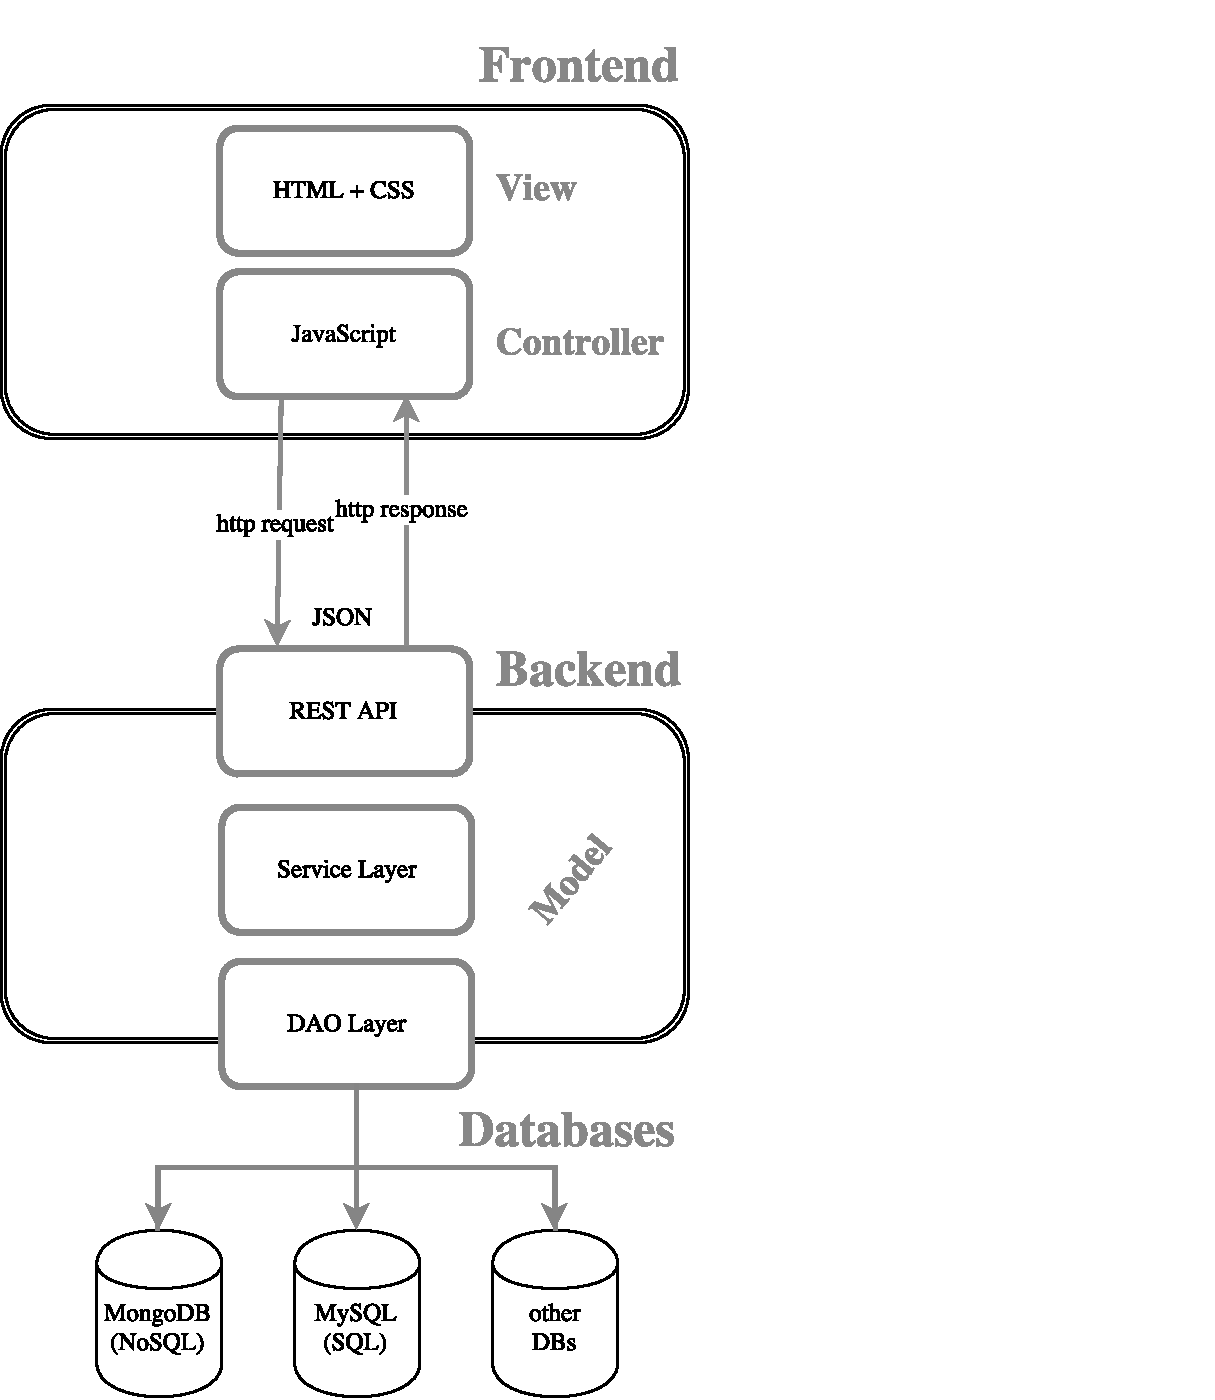
\includegraphics[trim = 0mm 0mm 0mm 0mm, clip, width=0.45\textwidth]{resources/architectureMyAppWithoutFrameworks}
\caption[Architektur-Prototyp]{Architektur-Prototyp}
\label{img:architectureMyApp}
\end{figure}

Die vorgeschlagene Architektur ist auf der Abbildung \ref{img:architectureMyApp} zu sehen. Die Auswahl dieser Architektur hat zum Einen das Ziel, ein möglichst gutes Skalierungsverhalten der Anwendung zu erreichen. Die für die Performance zwei kritischen Komponenten - Backend-Server und die Datenbank - werden auf mehreren Rechnern verteilt. Der entscheidende Faktor für das Skalierungsverhalten beider Komponenten ist, wann und wie viel Synchronisation notwendig ist. 

Zum Anderen wird das Ziel verfolgt, die Antwortzeit sowohl für die Anfragen, die Leseoperationen in der Datenbank benötigen, als auch für die Anfragen, bei denen die Daten gespeichert werden müssen, bei steigender Anzahl der Internetnutzer konstant zu halten.

\subsection{Backend}
%\subsection{\colorbox{green}{Backend}}

Der Backend stellt seine Funktionalität als eine Menge von Webservices mit \textit{REST}-Interface zu Verfügung.

\begin{figure}[H]
%\vspace{-20pt}%
\centering
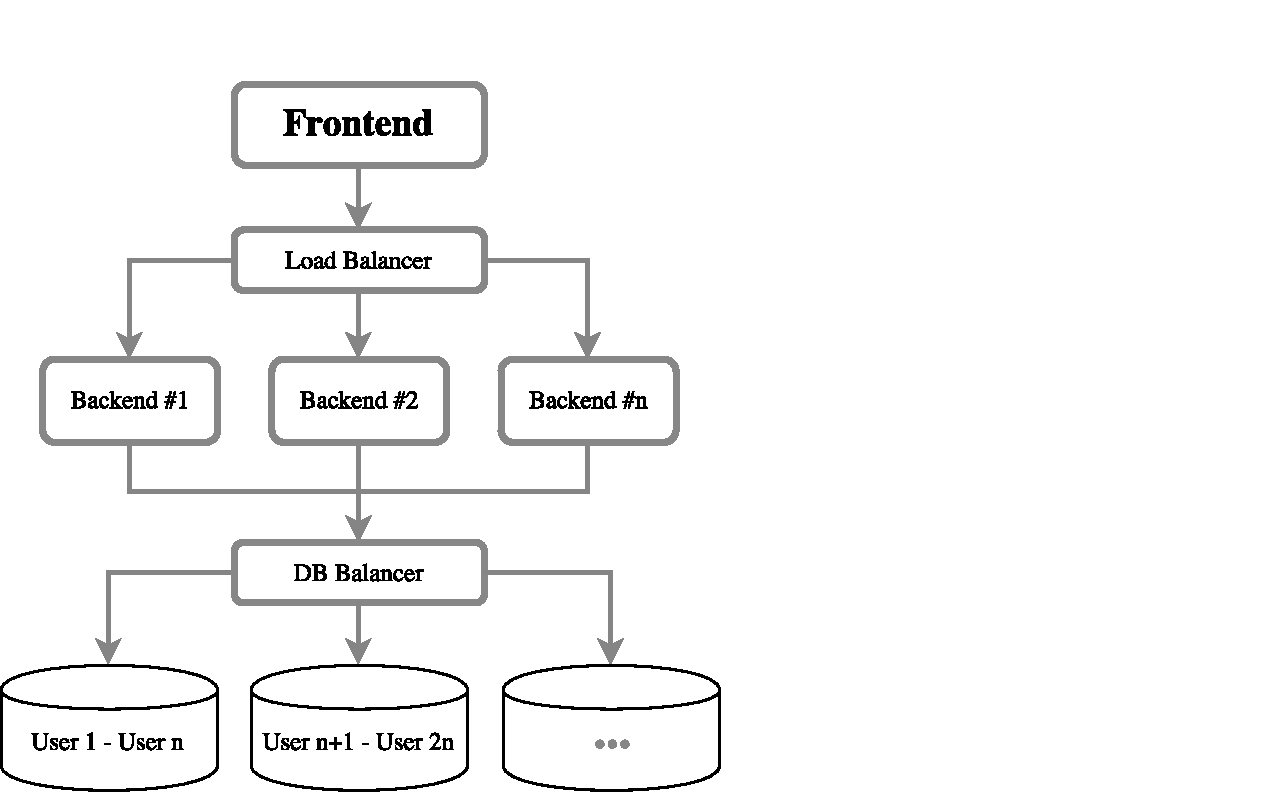
\includegraphics[trim = 0mm 0mm 0mm 0mm, clip, width=0.60\textwidth]{resources/ueberblickArchitektur}
\caption[Vorgeschlagene Architektur im Überblick]{Vorgeschlagene Architektur im Überblick}
\label{img:ueberblickArchitektur}
\end{figure}

Um ein gutes Skalierungsverhalten zu erreichen, wird jede Anfrage unabhängig von den anderen Anfragen bearbeitet. In dem Backend werden keine Informationen zwischengespeichert. Alles was gespeichert werden muss, wird in die Datenbank geschrieben. Solche Abläufe nennt man \textit{stateless}, weil sie keinen Zustand speichern. Somit ist keine Synchronisation zwischen den Maschinen des Backends notwendig, sogar die Anfragen innerhalb einer User-Session können von verschiedenen Maschinen bearbeitet werden. Ein \textit{Load Balancer} kann die Anfragen auf verschieden Maschinen in Backend verteilen ohne Rücksicht darauf nehmen zu müssen, welcher Maschine die jeweilige Anfrage entstammt.

Die Webservices sind unabhängig voneinander und können auch auf verschiedenen Maschinen ausgeführt werden. Diese Architektur ist auch als \textit{Microservice} Architektur bekannt.

%\subsection{\colorbox{green}{Datenbank}}
\subsection{Datenbank}

Das Skalierungskonzept für die Datenbank basiert auf der Annahme, dass die Webanwendung auf \textit{Multi-User} Betrieb ausgelegt ist und jeder User seine Daten unabhängig von den anderen Usern verwaltet. Daher ist es möglich, die Daten so aufzuteilen, dass sich alle Daten eines bestimmten Users nur in einem Teil der Daten wiederfinden. So kann jeder Teil der Daten getrennt von allen anderen Teilen, z. B. auf eigener Maschine, gespeichert werden. Wenn der Backend-Server eine Anfrage bearbeitet, sind die Daten nur eines Nutzers betroffen. Damit fragt der Backend-Teil nur die Komponente ab, die entsprechenden Teil der Daten verwaltet. Es ist notwendig, diese Komponente zu identifizieren. Jedoch ist es eine billige \textit{Mapping}-Abfrage, z. B. von dem UserID zu der IP-Adresse der Maschine, die die Daten verwaltet. Während des \textit{Live}-Betriebs ist auch keine Synchronisation erforderlich. Die Synchronisation ist nur dann relevant, wenn die Daten neu aufgeteilt werden müssen.

\section{Umsetzbarkeit}
%\section{\colorbox{yellow}{Umsetzbarkeit}}
Diese Architektur kann mit bereits beschriebenen Frameworks und Tools realisiert werden.

Der Frontend-Teil der Webanwendung kann als \textit{Single-page-Webanwendung} mit dem Einsatz des modernen Angular 2 - JavaScript Frameworks implementiert werden. Damit kann auch in Frontend objektorientiert entwickelt sowie die modulare Entwicklung durch \textit{Dependency Injection} unterstützt werden. 

Für \textit{Load Balancer} kommt beispielsweise der Einsatz von \textit{Nginx} \cite{nginx} infrage. \textit{Load Balancer} verteilt die Last auf mehrere Maschinen des Backends. Die Last wird auf dem Level der einzelnen Abfragen verteilt. 

Bei der Umsetzung des Web-Servers kann das Spring Framework benutzt werden. Mit dem Spring Framework werden mehrere Konzepte umgesetzt, so wie \textit{REST API}, \textit{Dependency Injection Pattern} und die Möglichkeit den Backend-Teil des Prototyps als ein \textit{Self-Contained} System zu betrachten.

Die Speicherung der Daten wird durch die \textit{NoSQL}-Datenbank \mongo\ realisiert. Für die Aufteilung der Daten einzelner Kollektionen in kleinere Teile wird das \mongo-Konzept \textit{Sharding} vorgenommen, um jeden Teil der Daten getrennt von allen anderen Teilen zu speichern, beispielsweise auf einem getrennten Server. Zusätzlich zum \textit{Shardings-}Konzept wird ein \textit{Replikations-}Konzept für den möglichen Serverausfall vorgesehen. Realisiert wird dieses Konzept mit Replikationsgruppen. Für jede Replikationsgruppe sind mindestens drei Server notwendig. Die Schreibzugriffe werden über einen einzigen Server erfolgen, die weiteren zwei Server stehen nur für die Replikation der Daten.
